\def\bibliocommand{\bibliography{bibliography}}
\input{latBegin.txt}

\part{Introduction}
\label{introduction}

\chapter{Our closest cousins}
\label{ourclosestcousins}

The kingdom Fungi is one of the most diverse groups of organisms on Earth, and they are integral ecosystem agents with a huge impact on biogeochemical cycles, plant and animal pathology, plant nutrition and soil properties.
While historically clustered together with plants ~\citep{copeland1938, copeland1956}, towards the middle of last century it started to become clear that this lumping failed to properly deal with the differences between the two groups. In 1969 R. H. Whittaker published a paper dividing the organisms into five kingdoms: Animalia, Plantae, Fungi, Protista and Monera ~\citep{whittaker1969}. By the 70s this division became widely accepted, and the Kingdom Fungi was recognized.
Acknowledgement is just the first step in knowledge though. The understanding of the taxonomy, evolution and phylogenesis of fungi was still a matter of ample debate, one of those that may never end for lack of evidence. All the analysis were based on morphological differences, with all of its downsides.

Fossilized fungi are very difficult to come by, as they do not biomineralize like animals do, and has proven not only inconclusive with regard to the origin of fungi, but also rather incomplete relative to the evolutionary history of the various fungal lineages. The earliest compendium of fossil fungi is from the late 19th century ~\citep{meschinelli1898}, and the symbiotic relationship with plants in fossils was suggested around that period ~\citep{renault1896}, but the difficulty in the interpretation of morphological data made it impossible to actually understand what happened.

Earliest fossil with the morphological features of a fungus is dated to around 1 billion years ago, and was found in the Arctic Canada ~\citep{loron2019}, and there is evidence of fungus-like organisms in fossils of around 800 Mya ~\citep{bonneville2020}. Those findings are rare though, we surely have a richer diversity of fossils from the lower Devonian (around 400 Mya).

It wasn't until the large scale advent of molecular phylogenetics techniques that some light could be properly shed on the history of fungi ~\citep{james2006}.
From molecular clock analysis seems like fungi are sister group to animals, that is, the two lineages are close, diverging around 1.5 Billion years ago ~\citep{wang1999}. The two groups form one supergroup called Opisthokhonta ~\citep{cavalier-smith1987}, from the Greek opísthios (rear, posterior) and kontós (``pole'' i.e. ``flagellum''), since the group is characterized by flagellate cells that propel themselves with a single, posterior flagellum (in many cases lost).

IMG OF TREE WITH ANIMALS AND FUNGI AND PLANTS

\chapter{Ancient lovers}
\label{ancientlovers}

So: fungi are animals' cousins, and the two lineage diverged around 1.5 billion years ago. What happened then?

The ancestors of fungi are believed to be simple aquatic forms with flagellated spores, similar to members of the extant phylum Chytridiomycota (chytrids), which are now considered one of the early-diverging clade in the kingdom ~\citep{james2006}. The first terrestrial fungi colonized land probably before plants did ~\citep{heckman2001}, as saprobe (taking nutrition out of dead matter) and\slash or in symbiosis with organisms capable of photosynthesis.
It is commonly accepted that in order to colonize the land, plants had to develop a symbiotic relationship with fungi ~\citep{selosse1998, heckman2001, bonneville2020}, but it is not entirely clear whether this relationship was lichen-like or mycorrhizal-like.

IMG LICHEN

Lichens are the symbiotic relationship between a singol or more fungi (\emph{mycobiont})and a cyanobacteria or algae (\emph{photobyont}). Think about an algae floating in water: for many reasons, it is not really equipped to deal with the challenges of a terrestrial life style: mainly, it won't be able to mine substrate resources, to protect itself against dehydration, constant direct UV radiations and strong temperature fluctuations ~\citep{selosse1998, blackwell2000}. In a lichen, the photobiont is protected by the fungal stroma, and it can tolerate drought, cold, heat, intense light and barren rocky substrates. They also seem to be the first pioneers in a barren environment today, so everything would point to them being the right candidate for a first out-of-water plant-fungi symbiosis.

Yet, while this relationship evolved several times ~\citep{gargas1995}, the only phyla we know that are capable of such process (called \emph{lichenization}) are Ascomycota and, secondarly and later in time, Basidiomycota, and we can date the origin of those clades to about 400 Mya in the Devonian ~\citep{berbee1993}. Similarly we have fossils for lichens dating at the oldest in the Early Devonian (400 Mya) ~\citep{taylor1997, honegger2013}, while the first fossil land plants and fungi appeared 480 to 460 Mya, and molecular clock estimates suggests about 600--700 Mya ~\citep{berbee1993, heckman2001}.

Therefore, lichens were likely not what opened the way to plants for land colonization. Let's look now at a mycorrhizal-like relationship.

Mycorrhiza is the symbiotic association between plants and fungi happening in the rhizosphere, that is, the plant's root system. It consist in an exchange of resources between the fungus and the plant, ideally the plant providing sugar to the fungus and the fungus providing minerals and nutrients to the plant, even though it's hard to pinpoint who's benefiting who and it may fall on different scales of the parasithic-mutualistic spectrum

What we know is that fossils resembling mycorrhizal relationships have fossil dating back to the Ordovician (with an age of about 460 million years), and are Glomales-like Arbuscular Mychorrhizal (AM hereafter) fungi, in a moment where the land flora is supposed to only consist of plants on the bryophitic level ~\citep{redecker2000}. Now, plants can photosynthetize; these fungi can extract minerals from the substrate with great efficiency, protect the root system, extend the range from which water can be taken and protect the plants from pathogens. It's easy to see how this is going to end up in a passionate love story.

You could say ``\emph{wait a minute: those plants did not have true roots, how can we have a mycorrhizal relationship?}''. Good point. Fossil records provides evidence that fungal organisms entered in such symbiosis before the appearance of true roots, and as long as there is a multicellular host AM fungi are fine ~\citep{wang2006, bonfante2008}.

Whether as lichen or as mycorrhiza, the symbiosis between plants and fungi is one of the most important, most ancient relationship in the history of living beings and it surely played a crucial role in the successful colonization of the land by plants ~\citep{pirozynski1975, malloch1980, harley1987, trappe1987, selosse1998, brundrett2002}. The relationship is so beneficial (for one or both parts) that today is the norm, and is well established in c. 85\% of extant plants ~\citep{cairney2000, strullu-derrien2018}, with a high degree of complexity ~\citep{heijden2015} and mychorrizas networks often constitute 20\%–30\% of total soil microbial biomass ~\citep{leake2011}

\chapter{Orchids}
\label{orchids}

Let's move the camera away from fungi for a second. Don't worry, we'll get back to them soon enough, but now we need to introduce the second protagonist of the present work: orchids.
Orchids are a diverse and widespread family of flowering plants, counting over 28,000 species in about 736 genera ~\citep{christenhusz2016}, second only to \emph{asteraceae} in terms of number even though they got on the scene only around 80 Mya ~\citep{ramirez2007}, not very long ago. They are cosmopolitan, with a distribution spanning all continents except Antarctica and including most major island groups ~\citep{givnish2016}.
By the end of 2017 the IUCN Global Red List included assessments for 948 orchid species, of which 56.5\% are threatened ~\citep{fay2018}. In Europe all wild orchids are protected, being included in their entirety on Appendices I and II of the Convention on International Trade in Endangered Species of Wild Fauna and Flora ~\citep{CITES-1} as are many of the habitats they live in, and are in many countries Red List. Nonetheless, this protection has not staved off a general decline in the orchid flora of Europe ~\citep{jacquemyn2005, kull2006}. Major threats include habitat destruction and unsustainable (often illegal) harvesting, and because of their complex life histories orchids are thought to be particularly vulnerable to the effects of global environmental change ~\citep{kull2016, gale2018}

Orchids exhibit an astonishing diversity of habitat adaptations, morphologies and pollination strategies, but some characteristics are common to the whole family. One of the most important is the reliance on Orchid Mycorrhizal Fungi (OMF hereafter) for reproduction and often outright survival. I told you we would soon get back to them.
Orchids seeds are devoid of nutritional resources, and they completely rely on fungi for nutrition including water, minerals and carbon supply ~\citep{leake1994, rasmussen1998, merckx2013} in a nutritional strategy called ``mycoheterotrophy''. After germination, seedlings often become autotrophic and subsequently revert to usual mycorrhizal functioning ~\citep{rasmussen1995, cameron2008}. Some species, especially from forest environments, remain mycoheterotrophic at adulthood though, developing partial photosynthetic capacity but still relying on fungi for carbon resources, a nutritional strategy called ``mixotrophy'' or ``partial mycoheterotrophy'' ~\citep{gebauer2003, julou2005, selosse2009}. Others never develop photosynthetic capacity and therefore rely completely on fungi for nutrition. This nutritional mode, which has evolved over 30 times independently in orchids, is called ``obligate mycoheterootrophy'' ~\citep{merckx2013}. So: no OMFs, no orchids.

While the relationship between orchids and OMFs is known since over a century ~\citep{bernard1899, rayner1927, rasmussen2002, selosse2011} and the mechanisms of this symbiosis are beginning to be properly understood, the knowledge from a taxonomical standpoint is still in full evolution. For many years orchids were thought to interact almost entirely with the members of the \emph{Rhizoctonia} complex. It was later discovered not only that orchids have way more interactions with different fungi also from the \emph{Ascomycetes} phylum, but also that \emph{rhizoctonia} is a polyphyletic group, and was disassembled in different taxa, all members of the \emph{Agaricomycetes}, most notably \textbf{\emph{Sebacinales, Ceratobasidiaceae}} and \textbf{\emph{Tulasnellaceae}} ~\citep{dearnaley2012}.
There is also evidence of fungi from the \emph{Ascomycota} phylum, especially in the order \emph{Pezizales} ~\citep{selosse2004, ouanphanivanh2008, waterman2011}, but they are the exception rather than the rule: the most common and known families of OMFs are in the \emph{Basidiomycota} phylum, especially \emph{Inocybaceae}, \emph{Tulasnellaceae}, \emph{Ceratobasidiaceae}, \emph{Russulaceae}, \emph{Sebacinaceae}, \emph{Serendipitaceae} and \emph{Thelephoraceae} ~\citep{taylor2004, roy2009, duffy2019}

\section{Distribution and ecology of OMFs}
\label{distributionandecologyofomfs}

Since as we've seen orchids depend on OMFs for the germination of the seeds and in many cases for the nutrients also in adulthood, it is safe to assume that OMFs are everywhere orchids are. This is not the whole tale though, as we know that many OMFs can also turn to a soil free-living saprotrophic ecological niche ~\citep{oberwinkler2017} and form mycorrhizal relationship with plants other than orchids ~\citep{selosse2014}, allowing them to spread to a bigger area. \emph{Tulasnellaceae, Ceratobasidiaceae,} and \emph{Sebacinales}(\emph{Serendipitaceae} and \emph{Sebacinaceae}) are ubiquitous, varying in their contribution to the total amount of OMFs depending on the area and in the level of specialization for the orchids. Other families, even though less common, still have a presence in most of the world ~\citep{jacquemyn2017}.

This is all good and well as long as we look at the matter a broad scale. Here, the abiotic variables such as annual rainfall, soil chemistry etc. explain the distribution the best, but when we zoom at a more local level biotic factors, community composition and interactions may affect the OMFs distribution just as much, especially considering they are symbiotic organisms ~\citep{jacquemyn2017}. I used \emph{may}, as there is a lack of evidence in this regard, and many parts of the world are dramatically undersampled (e.g. all the African continent and most of the tropical areas of the planet), so conclusions are often drew from a limited amount of very specific data. Part of the ``problem'' is how complex the relationships between orchids and OMFs are. They both vary in their degree of specialization, from a highly specialized to a more generalist approach ~\citep{mccormick2004, girlanda2011, heijden2015}, and OMFs can also turn to other ecologies, as pathogenic fungi and saprophitic free-living organisms ~\citep{veldre2013}.
The community question it's critical: do OMFs from different families occour in different habitats? How much do the biotic factors impact the OMFs distribution compared to abiotic factors?
Do OMFs belonging to the same family occour in different habitat? How much does is the preference for an habitat a shared characteristic for a group?
Giving a partial answer to those questions, in regard to Europe, is the main aim of the present work.

\part{Materials and methods}
\label{materialsandmethods}

\chapter{The database}
\label{thedatabase}

Data from bibliography regarding the distribution of OMFs in Europe was collected into a starting database. The data had to be of fungi isolated from known orchid roots, and had to be georeferenced at the very least with the name of a close enough place; also, each sample had to have a genbank accession code in order to get the sequences and do the analysis.
Only sequences from well-known OMFs were considered, that is: Ceratobasidiaceae, Tulasnellaceae, Inocybaceae, Serendipitaceae, Sebacinaceae, Russulaceae and Thelephoraceae ~\citep{dearnaley2012}.
Orchid species sampled were Orchis anthropophora, Cephalanthera damasonium ~\citep{julou2005}, Cephalanthera longifolia ~\citep{pecoraro2017}, Orchis simia and Orchis simia ~\citep{schatz2010, lievens2010}, Orchis tridentata ~\citep{pecoraro2012}, Orchis militaris ~\citep{shefferson2008}, Orchis purpurea ~\citep{lievens2010}, Himantoglossum adriaticum ~\citep{pecoraro2013}, Limodorum abortivum ~\citep{girlanda2005}, Spiranthes spiralis ~\citep{duffy2019}, Ophrys bertolonii ~\citep{pecoraro2015}, Neottia ovata ~\citep{hansjacquemyn2015, tesitelova2015} Neottia cordata ~\citep{tesitelova2015}, Dactylorhiza baltica ~\citep{shefferson2008} and Epipactis atrorubens ~\citep{shefferson2008}

For each point six variables were extracted by using the ESDAC database ~\citep{esdac} and the World Clim database ~\citep{worldclim}: Nitrogen, Potassium and Phosphorus soil content, soil pH, minimum temperature of the coldest quarter and maximum precipitation of the wettest month. Those variables were selected because there is evidence that mycorrhizal fungi are very sensitive to nutrients in the soil: Nitrogen, Phosphorus and Potassium in high quantities (such as in eutrophicated soils because of agricultural fertilizers) have been seen to cause decline in the belowground mycorrhizal fungi species richness and cause dramatic changes in the community composition and structure ~\citep{lilleskov2002, baar2002, grant2011}. Mycorrhizal fungi growth and community composition also seem to be influenced by the soil pH ~\citep{aarle2002, carrino-kyker2016}, temperature and precipitation ~\citep{rillig2003}. That's not all though: those variables may serve as important proxy for other conditions. Biomes and vegetation are correlated with the environmental condition, both because they change said conditions (like soil pH) and because all species have a range of tolerance. Also, human impact can often be seen by the amount of chemicals in the soil, especially close to cultivated fields.
Environmental values were extracted using \texttt{GDAL}'s \texttt{Sample Raster Values} tool (Using QGIS v. 3.16 as a GUI) and appended to the dataset

\begin{figure}[htbp]
\centering
\includegraphics[keepaspectratio,width=\textwidth,height=0.75\textheight]{images/map.png}
\caption{Sampled points}
\end{figure}

\chapter{Phylogenetic analysis}
\label{phylogeneticanalysis}

In order to understand the distribution and ecology of the OMFs we need to get a better insight of their phylogenesis. The hypothesis was for sequences of the same family to be clustered together, with some doubts with the Sebacinales as Serendipitaceae and Sebacinaceae are very close and only recently named so ~\citep{weiss2016}.
The phylogenetic analysis were performed on the sequences deposited by the papers included in the database.
The \textbf{primers} used were mainly ITS1F, ITS4, ITS3 and ITS4OF, all targeting \textbf{regions} between the 18S rRNA subunit and the 28S rRNA subunit, including the Internal Transcribed Spacers (ITS hereafter) 1 and ITS 2. Those primers were usually universal for \emph{Basidiomycota} or in some cases more specific for \emph{Tulasnellaceae} (like ITS4tul) or other taxa.
Sequence \texttt{DQ520100} from \emph{Tremiscus helvelloides} was used as outgroup.

\begin{itemize}
\item Sequences were aligned using the MUSCLE algorithm ~\citep{edgar2004} and manually trimmed to a visually satisfying overlapping

\item Ugene was used as main GUI, v. 37.0 ~\citep{okonechnikov2012}

\item The Maximum Parsimony analysis was performed using TNT, v. 1.1 ~\citep{tnt}, using the Tree Bisection and Reconnection algorhithm and with ten replics. 1000 trees were kept and a strict consensus tree was calculated. A bootstrap was performed on the tree with 200 replications to test the validity of the tree. Bootstrap values are displayed as node labels in the appendix tree

\item The Bayesian analysis (MCMC) was performed using MrBayes, v. 3.2.7a ~\citep{huelsenbeck2001}, using the Hasegawa-Kishino-Yano with a gamma rate heterogeneity among sites (\texttt{lset nst=2 rates=gamma;}). One million trees were generated and sampled each thousand, with four chains running. A final consensus tree was then calculated (see appendix)

\item Trees were then visually edited with FigTree v. 1.4.4

\item All parameters are available in the supplemental data, along with the files to reproduce the analysis.

\end{itemize}

\chapter{Multivariate analysis}
\label{multivariateanalysis}

Before proceeding with the multivariate analysis, sequences have been clustered into Operative Taxonomic Units (\textbf{OTU} hereafter), by using cd-hit v. 4.8.1 ~\citep{li2001}. This process yielded 210 OTUs, with the extremes of \emph{Serendipitaceae} having two OTUs only, and \emph{Tulasnellaceae} 52 OTUs.
The database was then pivoted in a presence-absence matrix, and for further analysis it was splitted by family, so that each matrix only had all the OTUs for that single family, yielding 7 different matrices. This was necessary to test what internal variability each family has; another matrix was obtained by grouping together all the observations from the same family, to test what the variability between the different families is.

\begin{figure}[htbp]
\centering
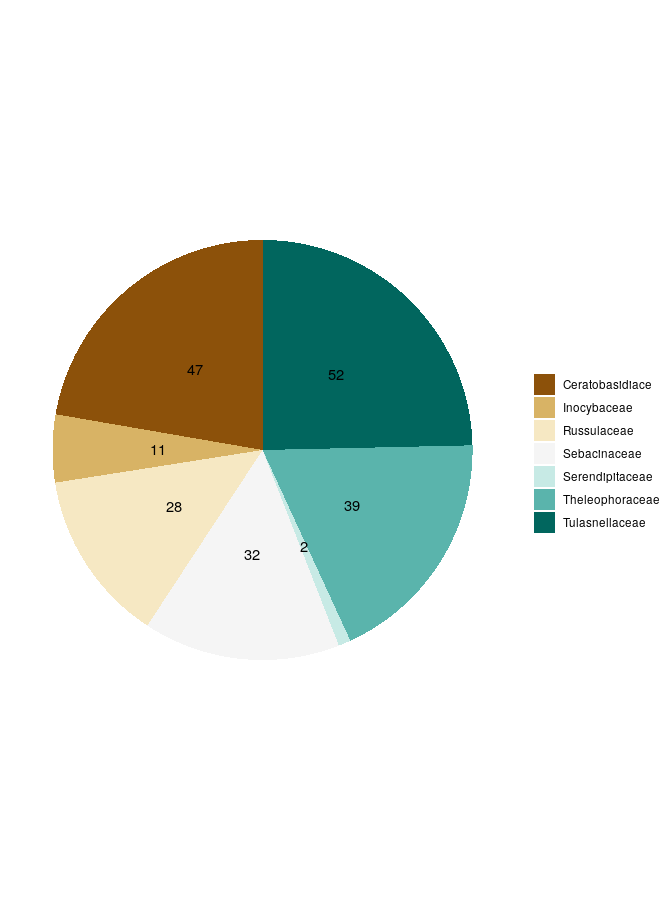
\includegraphics[keepaspectratio,width=\textwidth,height=0.75\textheight]{images/clust.png}
\caption{Number of OTUs from each family}
\end{figure}

A final matrix was obtained by using the single Families\slash OTUs as rows and removing the qualitaties orchid species variable. This was done to understand the impact of the environmental variables only on each OTU, therefore trying to understand how different the realized niche (ie variance in the environmental variables) is between the groups.

Principal Component Analysis (PCA hereafter) is an orthogonal linear transformation of the data that aims to maximize the variance of the scalar projection of all points of a dataset into a number of axis ordinated by explained variance. This yields a set of axis, which can be used for clustering, to reduce the number of dimensions and so on. PCA was performed on all matrices using the base R functions \texttt{princomp()}, which takes into account the covariance matrix and applies an eigen method of spectral decomposition when possible. Only in the case of Russulaceae, when the number of observation was too limited, \texttt{prcomp()} was used, which does a single value decomposition on the centered and scaled data matrix.

As of clustering, Non-metric Multi Dimensional Scaling (NMDS) is another widely used method that allows to visualize the level of similarity of individuals in a dataset. In contrast with PCA, it's non-linear and it's based on a distance matrix, computed by different algorithms depending on the data. It works better with non-parametric data, such as the present one. NMDS was performed on all the matrices by using the R package \emph{vegan} ~\citep{dixon2003a}, to understand both how do the OTUs from different families cluster together (if they do) and what environmental factors are most relevant; the Euclidean distance method was used.

In both the PCA and the NMDS we have taken into account how each OTUs presence was influenced by environmental factors, such as climate and soil conditions, and how do they cluster together.
Species Distribution Models (SDM hereafter) is another conceptual framework we can use to disentangle the assembly processes that lead to the community as we can observe from the data we have, and to infer the relative importance of the environmental factors. SDMs are numerical tools that combine observations of species occurrence or abundance with environmental estimates. They are used to gain ecological and evolutionary insights and to predict distributions across landscapes, sometimes requiring extrapolation in space and time ~\citep{elith2009}; those models can also inform us of how species‐to‐species associations depend on the environmental context, in a Joint Species Distribution Model which oftentimes outperforms simple SDMs especially with sparse data ~\citep{pollock2014, tikhonov2017}

In the present work, a kind of JSDM called Hierarchical Model of Species Community (HMSC) ~\citep{ovaskainen2017} was performed by using the \texttt{Hmsc} package in R, v. 3.0.9 ~\citep{tikhonov2020, hmsc-r2021}; this method uses a bayesian framework to find the best fitting model based on the data, and works very well with presence-absence data as well as with environmental data ~\citep{hefley2016}
Three parallel chains were run, sampling every 500 results. Regression was done with a probit model (probability + unit), a non-linear model where the dependent variable can only take two variables, which was particularly apt for this dataset because of the binary nature of the presence-absence matrix.
Using this framework, a plot with the species responses to environmental covariates (beta parameters) was produced, with at least a 85\% posterior probability of being positive (red) or negative (blue).
In addition, by using the presence-absence matrix, a correlation plot between the OTUs was established, looking at the positive associations with a statistical support of at least 85\% shown in red and negative associations shown in blue.

\part{Results}
\label{results}

\chapter{Phylogenetic analysis}
\label{phylogeneticanalysis}

The \textbf{Bayesian analysis} yielded low probability branches. Nonetheless, it correctly put together the families, with the only notable exception of the \emph{Serendipitaceae} and \emph{Sebacinaceae} which were nested separately. This makes sense though, as they are both \emph{Sebacinales} and the \emph{serendipitaceae} were originally considered \emph{sebacinaceae B} ~\citep{weiss2004} and were only recently given a new name and properly defined ~\citep{weiss2016}
The \textbf{Maximum parsimony analysis} gave similar results, with very low bootstrap support

\chapter{PCA}
\label{pca}

The \textbf{PCA analysis} on the presence-absence matrix and the environmental variables combined showed how there is a substantial overlap of realized niche in the OTUs isolated from different orchids, without distinguishable clusterings except for the Tulasnellaceae isolated from Neottia cordata.
In all cases, the variance was well explained by the first two components (>95\% explained variance), with two variables bearing most of the loading: Maximum Precipitation of the wettest month and Potassium content in the soil.

The PCA done using the condensed family matrix yielded the same results, with the notable exception of the Limodorum abortivum, which a way higher variance than expected 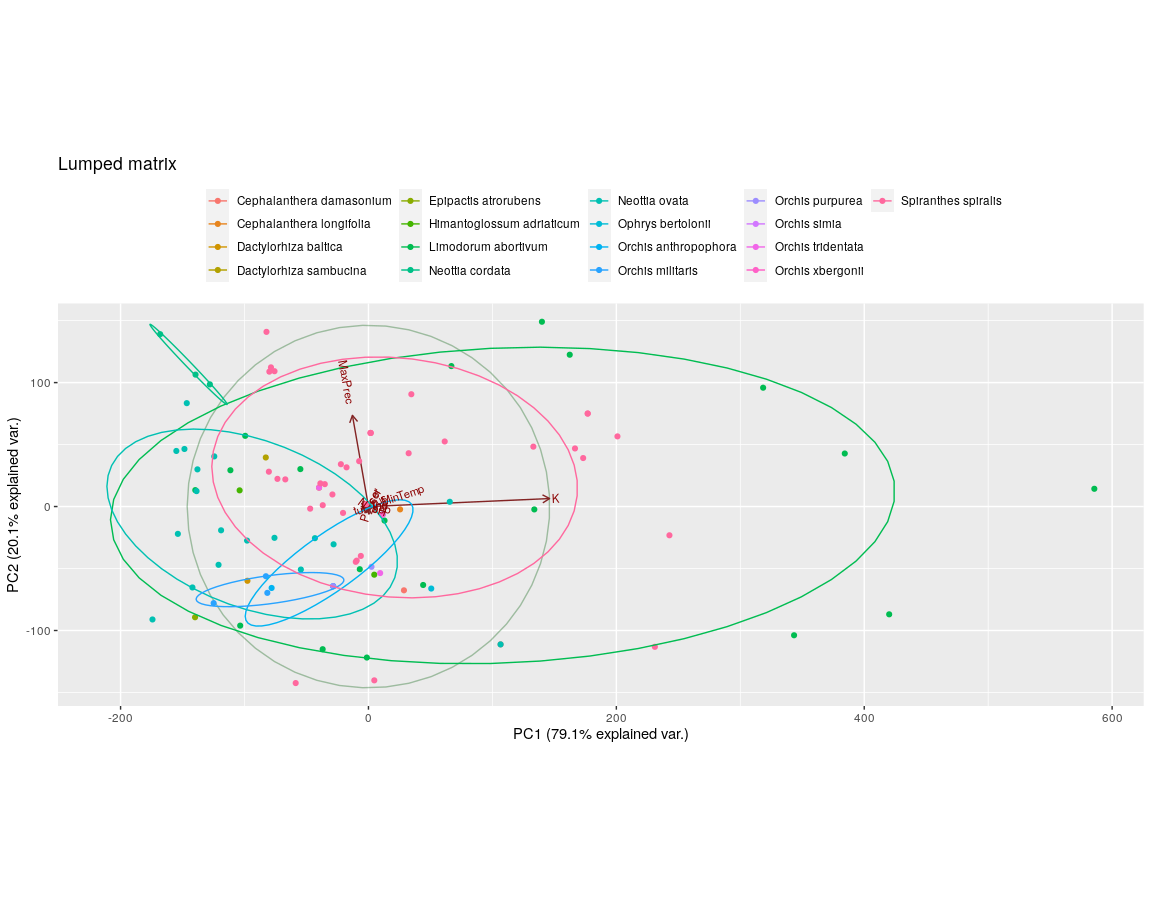
\includegraphics[keepaspectratio,width=\textwidth,height=0.75\textheight]{images/lumpPCA.png}

\begin{verbatim}
Condensed Matrix

          PC1      PC2
K         0.996
MaxPrec           0.994


Ceratobasidiaceae

         PC1      PC2
K       -0.991  0.117                                                                                                                                                 
MaxPrec  0.120  0.992  

Russulaceae

         PC1      PC2
K        0.995                                                                                                                        
MaxPrec        -0.994 


Theleophoraceae

          PC1    PC2
K        0.999                                                                                                                        
MaxPrec         0.987
\end{verbatim}

\chapter{NMDS}
\label{nmds}

The \textbf{NMDS analysis} on the single families seems to show that there is no highly relevant differentiation in the OTUs found in different orchid species, as the clustering wasn't really neat.
Again, Tulasnellaceae seem to be the exception, with more distinct groups for different orchid hosts; while this could be a bias caused by the higher number of samples, Ceratobasidiaceae and Theleophoraceae did not show this pattern even though the sample amount where roughly similar. This could point to a higher specialization of the Tulasnellaceae group, confirming previous observations ~\citep{dearnaley2007}
The NMDS campiring the families yielded only a partial overlapping clustering, which could indicate that different orchids may have different degrees of specialization and realized niche; Limodorum abortivum seemed to exibit the highest diversity, together with Spiranthes spiralis.

Taking the Orchid species out of the NMDS analysis and only looking at how different OMF families clustered based on the environmental conditions showed an unexpected pattern. Russulaceae seemed to have a way bigger variance, which points to a broader realized niche, compared to all other families; Tulasnellaceae, which is the most sampled and abundant OMF in the dataset, had less than half the variance and clustered in an area comparable to Sebacinaceae.

\begin{figure}[htbp]
\centering
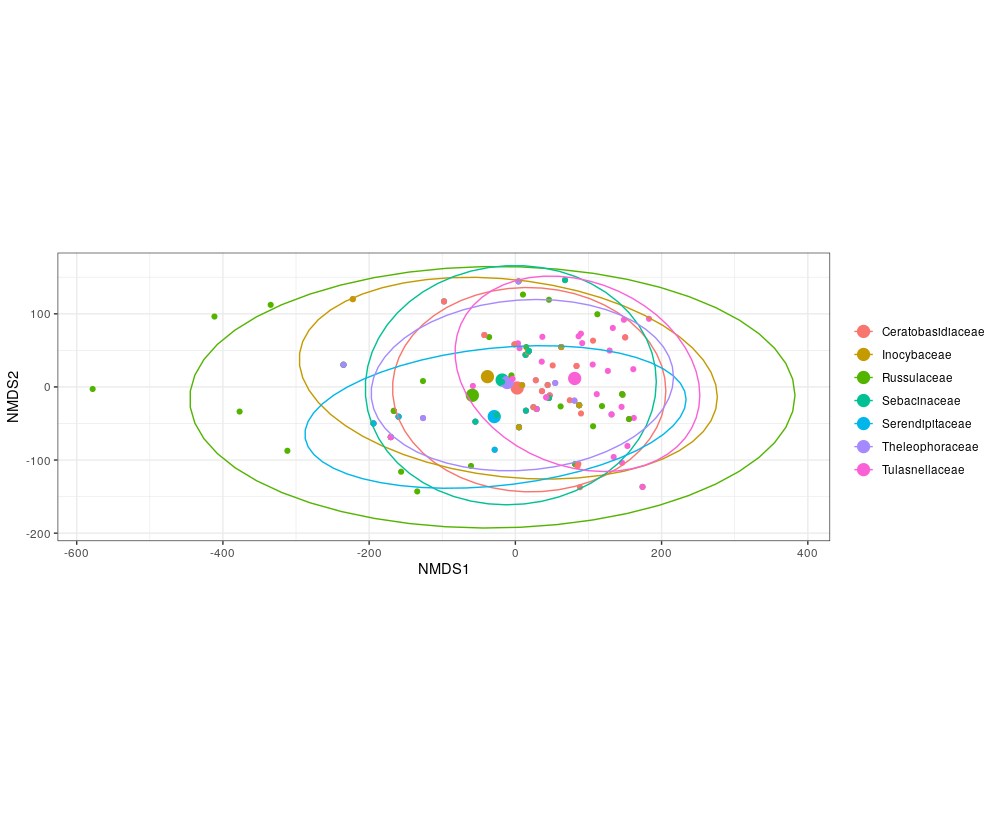
\includegraphics[keepaspectratio,width=\textwidth,height=0.75\textheight]{images/nmdsEnvMatrix.png}
\caption{NMDS of the OMFs families considering environmental variables only}
\end{figure}

\chapter{HMSC}
\label{hmsc}

The \textbf{HMSC} yielded basically two results.
In the correlation between the families seemed like most families had a positive correlation, with two exceptions: Tulasnellaceae, who had no correlation (0) and Russulaceae, that had a negative correlation (-1). Apparently, Russulaceae not only have a bigger niche, they also don't share it. The mechanisms and reasons for such negative correlation could be interesting matter for future studies.
OTUs from the same families seemed, on the other hand, to have no correlation with the others, positive or negative. This stands true for all families but Ceratobasidiaceae, which had more complex correlations, both positive and negative. Whether this is phylogenetically related is to be understood.

\begin{figure}[htbp]
\centering
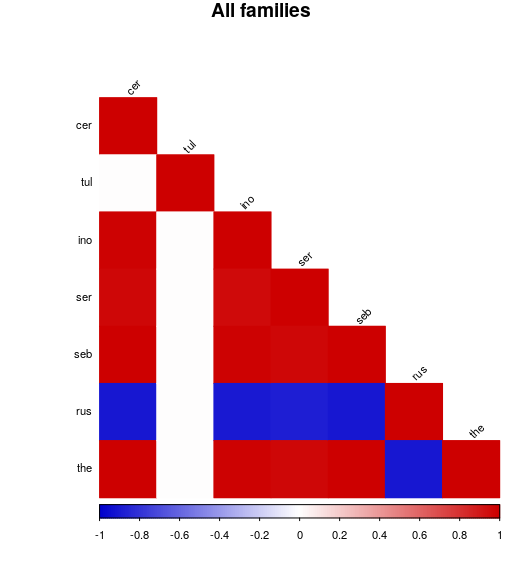
\includegraphics[keepaspectratio,width=\textwidth,height=0.75\textheight]{images/corrLump.png}
\caption{HMSC correlation between the families, taking into account the presence-absence data}
\end{figure}

\begin{figure}[htbp]
\centering
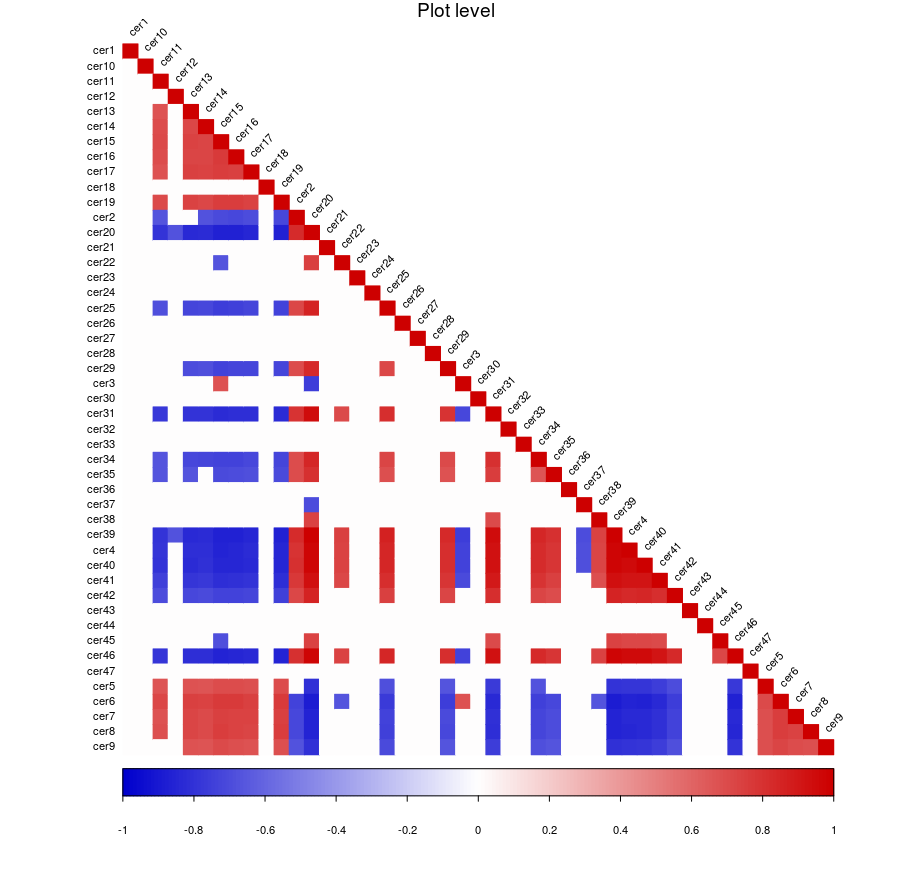
\includegraphics[keepaspectratio,width=\textwidth,height=0.75\textheight]{images/corrCer.png}
\caption{HMSC correlation between Ceratobasidiaceae OTUs}
\end{figure}

The second HMSC result is the correlation between the groups and the environmental variables.
The difference between the families wasn't very pronounced, and the most relevant parameter seemed the minimum temperature, which was highly correlated with most families (only Tulasnellaceae had 0 correlation), confirming the importance of this environmental parameter in understanding the distribution of OMFs. Maximum precipitation was also invertedly correlated with most families, except for Russulaceae which showed a positive correlation. Of all the soil parameters, pH seemed the most important with a general inverse correlation (the lower the pH, the higher the presence of the OMF).
The differences between OTUS from the same families were less clear-cut, showing different correlations for different OTUs in the same family, giving an idea of the diversity that can happen also at low taxonomic levels.
It's worthy of notice that Tulasnellaceae showed again the least amount of internal differences, with Ceratobasidiaceae being at the opposite side of the spectrum.

\part{Discussion}
\label{discussion}

The phylogenetic analysis yielded low quality trees, from which no useful data could be extracted. This is likely the result of the inconsistent overlap of the sequences. Many primers were used, and the resulting sequences were differently trimmed before depositing, with many partial sequences.

The PCA analysis was more fruitful. Together with NMDS it seemed to cluster together the fungi isolated from different orchid species, which would support the idea of the OMFs generalist approach as being the most common, which is a still ongoing debate ~\citep{bailarote2012}. Also, variance was mainly explained by two main variables, Potassium and Maximum Precipitation, which means that those variables contribute the least to the definition of the niche and that the Orchids were living in places highly differenciated in those parameters. This could also be the result of the very broad sampling, and more research should be done on a smaller scale, as the Potsassium levels can dramatically vary even in a very small plot, doubling in just a few meters ~\citep{bogunovic2014}.

Russulaceae seemed from the NMDS to be more tolerant than other families to different environments, and despite the lower number of sampled individuals we witness a more widespread. This could mean that the Russulaceae are more generalist toward orchids, that they have a wider niche or that it's more ecologically flexible, or all of the above. Russulaceae are a very diverse family, but it is actually difficult to say that Russulaceae find a ``niche'' in the symbiosis with orchids, especially with Limodorum, as there doesn't seem to be any advantage for the fungus: this orchids seem to have an insufficient photosynthesis and to heavily rely on the OMFs to provide not only minerals but also carbon-base chemicals; this also means that distribution of Limodorum may also be potentially constrained by the occurrence of its fungal symbionts ~\citep{girlanda2005}.

The HMSC put the spotlight on Russulaceae again, with their negative correlation with the other families. This means that where we find Russulaceae, we are unlikely going to find other OMFs. This is probably the result of the main orchid species where Russulas were found in this dataset, Limodorum abortivum, which seems to show a specialization toward this family ~\citep{girlanda2005}. The rest of the data seem to confirm a major generalistic approach in the recruitment by orchids, also confirmed by the lack of any correlation between the different OTUs of the same family: the presence of one doesn't seem to inhibit other OTUs from the same family to infect the root.

\input{latEnd.txt}


